\documentclass[article]{jss}
%\usepackage[T1]{fontenc}
%\usepackage[latin9]{inputenc}
%\usepackage{url}
%\usepackage{graphicx}
%\usepackage[authoryear]{natbib}
%\usepackage{babel}
%\usepackage{fullpage}
%\usepackage{hyperref}
%\newcommand{\pkg}[1]{{\fontseries{b}\selectfont #1}}

%%%%%%%%%%%%%%%%%%%%%%%%%%%%%%
%% declarations for jss.cls %%%%%%%%%%%%%%%%%%%%%%%%%%%%%%%%%%%%%%%%%%
%%%%%%%%%%%%%%%%%%%%%%%%%%%%%%

%% almost as usual
\author{Xiaoyue Cheng\\Iowa State University \And 
        Dianne Cook\\Iowa State University \And
        Heike Hofmann\\Iowa State University}
\title{\pkg{MissingDataGUI}: A Graphical User Interface for Exploring 
	Missing Values in Data}

%% for pretty printing and a nice hypersummary also set:
\Plainauthor{Xiaoyue Cheng, Dianne Cook, Heike Hofmann} %% comma-separated
\Plaintitle{MissingDataGUI: A Graphical User Interface for Exploring 
	    Missing Values in Data} %% without formatting
\Shorttitle{\pkg{MissingDataGUI}: Exploring Missing Values in Data} %% a short title (if necessary)

%% an abstract and keywords
\Abstract{
  Missing values are common in data, and usually require attention in order to conduct statistical analysis.  One of the first steps is to explore the structure of the missing values, and how missingness relates to the other collected variables.  This article describes an \proglang{R} package, that provides a graphical user interface (GUI) designed to help explore the missing data structure and examine the results of different imputation methods. The GUI provides numerical and graphical summaries conditional on missingness, and includes  imputations using fixed values, multiple imputations and nearest neighbors.
}
\Keywords{missing values, imputation, exploratory data analysis, 
	  statistical graphics, data visualization, graphical user interface}
\Plainkeywords{missing values, imputation, exploratory data analysis, 
	statistical graphics, visualization, graphical user interface}

%% publication information
%% NOTE: Typically, this can be left commented and will be filled out by the technical editor
%% \Volume{50}
%% \Issue{9}
%% \Month{June}
%% \Year{2012}
%% \Submitdate{2012-06-04}
%% \Acceptdate{2012-06-04}

%% The address of (at least) one author should be given
%% in the following format:
\Address{
  Xiaoyue Cheng\\
  Department of Statistics and Statistical Laboratory\\
  Iowa State University\\
  2406 Snedecor Hall\\
  Ames, IA, 50011, United States of America\\
  E-mail: \email{xycheng@iastate.edu}\\
  URL: \url{http://xycheng.public.iastate.edu/}\\
  \\
  Dianne Cook\\
  Department of Statistics and Statistical Laboratory\\
  Iowa State University\\
  2415 Snedecor Hall\\
  Ames, IA, 50011, United States of America\\
  E-mail: \email{dicook@iastate.edu}\\
  URL: \url{http://dicook.public.iastate.edu/}\\
  \\
  Heike Hofmann\\
  Department of Statistics and Statistical Laboratory\\
  Iowa State University\\
  2413 Snedecor Hall\\
  Ames, IA, 50011, United States of America\\
  E-mail: \email{hofmann@iastate.edu}\\
  URL: \url{http://hofmann.public.iastate.edu/}\\
}
%% It is also possible to add a telephone and fax number
%% before the e-mail in the following format:
%% Telephone: +43/512/507-7103
%% Fax: +43/512/507-2851

%% for those who use Sweave please include the following line (with % symbols):
%% need no \usepackage{Sweave.sty}

%% end of declarations %%%%%%%%%%%%%%%%%%%%%%%%%%%%%%%%%%%%%%%%%%%%%%%


\begin{document}

\section{Introduction}\label{introduction}

Missing values are a very common problem affecting data analysis. Many imputation methods are developed but little has been done for exploring the missing value structure visually.  Most plotting methods handle missing values by simply removing the incomplete records with or without a warning, especially when the data are continuous. Most statistical functions provide a limited list of handling missing values, such as delete all cases with missing, delete pairwise or on single variables only.

The issue is that in order to decide what to do with the missing values before analyzing the data, we need to understand what the distribution of the missing values is, and how the missingness depends on the other collected variables. A few \proglang{R} packages, like \pkg{Hmisc} \citep{hmisc}, \pkg{norm} \citep{norm}, and \pkg{mice} \citep{mice}, have some routines for summarizing the number of missing by variable, and by case, in preparation for imputing the missing values. To understand the distribution of missings versus non-missings we need to make plots of the data.

On the other hand, for some model-based imputation methods, it is important to check the assumptions, like missing completely at random (MCAR) or missing at random (MAR), but they are not easy to verify. \citet{little1988test} provided the tests for MCAR under the normal assumption, and \citet{jaeger2006testing} proposed an MAR test under the distributional assumption. Both tests employed the likelihood inferences, and gave the caution that the tests for MAR and MCAR are sensitive to model misspecification \citep{little1988test}, or MAR is non-testable \citep{jaeger2006testing}. Currently we do not find any \proglang{R} packages that can directly check the missingness assumptions, so a visual check will have some advantages - it may not confirm any randomness assumption, but it helps to deny the MCAR, or suggest the conditioning variables for MAR.

Some existing work describing the types of plots to explore missing data, and implementations, can be found in \citet{unwin1996interactive}, \citet{swayne1998missing}, and \citet{templ2008visualization}. First two of them use interactive graphics to help with the exploration. \proglang{MANET} implements the methods described in \citet{unwin1996interactive}. It presents the segmented barcharts of missing versus non-missing values for each variable. Since it has many plot types like histograms, scatterplots, mosaic plots, \proglang{MANET} encourages the user to select cases that are missing on any variable which highlights these cases in other plots enabling the user to explore the missing status dependence in the distributions of the complete cases of other variables.  \proglang{XGobi}, which implements the ideas described in \citet{swayne1998missing} provides more real-valued data tools. It creates a shadow matrix of the original data where entries are 0 (complete) or 1 (missing value). This additional data structure allows the user to explore the multivariate pattern of missing values, and to explore dependence between missing value status and distribution of the complete cases. Again, linked brushing is used, and rudimentary imputation methods are available in \proglang{GGobi} \citep{STLBC03}.

In the \proglang{R} community, package \pkg{VIM} \citep{VIM} provides a graphical user interface via \pkg{VIMGUI} \citep{VIMGUI}, to explore the structure of missing values and quality of several single imputation methods (kNN, hotdeck, irmi). Some packages for multiple imputation have interfaces for easy manipulation. For example, \pkg{migui} \citep{migui} is an interface for \pkg{mi} \citep{mi}, which implements multiple imputation via Bayesian models and weakly informative prior distributions; function \code{AmeliaView()} in \pkg{Amelia} \citep{amelia}, would generate a graphical interface, to implement its ``EM with bootstrapping'' algorithm. Meanwhile the package \pkg{miP} \citep{mip} adopts \pkg{VIM} to visulize the imputation results from packages \pkg{mice}, \pkg{mi}, and \pkg{Amelia}.

This current work describes a new package for \proglang{R}, \pkg{MissingDataGUI}, which allows the exploration of missing values structure, and comparison among the imputation results, using static graphics and numerical summaries. A GUI makes it accessible to novice users. This work builds on the ideas developed in \citet{unwin1996interactive} and \citet{swayne1998missing}. Meanwhile, the package utilizes routines in \pkg{Hmisc}, \pkg{norm}, \pkg{mice}, and \pkg{mi} for multiple imputation, with several other routines including kNN and random sample for the single imputation. The paper is structured as follows. Section \ref{Functionality} shows the design of GUI and explains what is done in GUI and why. Section \ref{Examples} gives an example. The last section discusses future work.


\begin{center}
\begin{figure}[h]
\begin{centering}
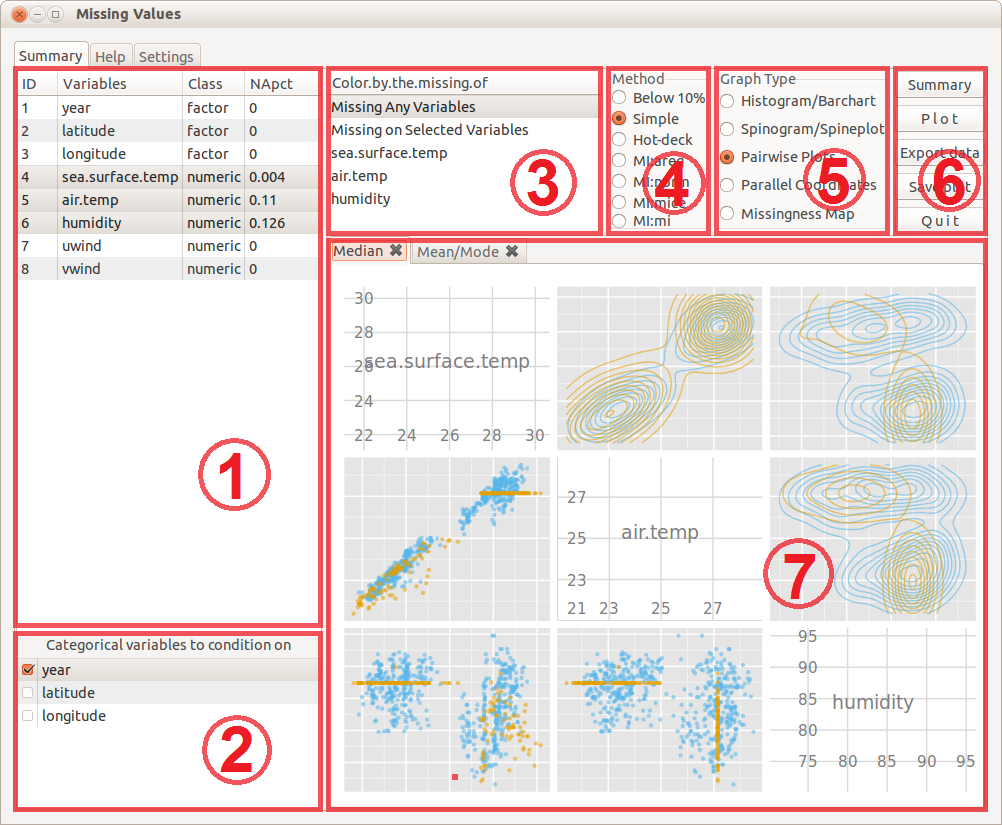
\includegraphics[width=.9\textwidth]{graph/fig1-GUI-tab1}
\par\end{centering}
\caption{Overview of the missing data GUI. Region 1 contains the list of variables, variable type, and summary of missings on that variable. Region 2 has a list of the categorical variables that can be conditioned on. Region 3 lists the variables having missing values, to enable coloring by different types of missingness in the plots. Region 4 contains a radio button selection of imputation methods. Region 5 has several plot type selections, and section 6 allows selecting numeric or graphical summaries and some output routines. The summaries are displayed in the region 7.}
\label{fig:missingGUI}
\end{figure}
\par\end{center}

\section{Functionality}\label{Functionality}

\subsection{Overview of the missing data GUI}

The missing data GUI looks as Figure~\ref{fig:missingGUI}. Section \ref{Examples} introduces the dataset. All variables with the classes and the percentages of \code{NA}'s are listed on the top left (area 1). The categorical variables, auto-detected by their classes, are shown on the bottom left as the potential conditions (area 2). The variables having missing values are displayed under ``Color.by.the.missing.of'' on the top center (area 3). The graphical summary will distinguish the imputations from the observations by two colors, yellow versus blue. This panel is used to name the variables that will determine the color. Selecting the first row ``Missing Any Variables'' means that the color will depend on whether the case has missing values in any variables. The second row ``Missing on Selected Variables'' means the graph is colored by whether the case has missings in the variables selected in area 1. ``Method'' (area 4) and ``Graph Type'' (area 5) are two widgets illustrated in section \ref{imputation} and \ref{plottype}. On the top right (area 6) there are five buttons: ``Summary'' can create a window as described in section \ref{numsum}; ``Plot'' produces the plots in the graphics panel on the bottom right of GUI (area 7); ``Export data'' saves the imputed data into a file or to \proglang{R} console; ``Save plot'' saves the plots in area 7 to png files; ``Quit'' destroys the main GUI window and the derived child windows.

\subsection{Summary of missing values}\label{numsum}

To investigate missingness in a data set, numerical summaries of the missings should be presented. As Figure~\ref{fig: num-summry} shows, the ``Summary'' button will open a window with the overall missingness information (left panel) or conditioning summary (right panel), depending on whether the conditioning variables are chosen in area 2. Both summary windows present the percent of the values that are missing, the percent of variables that contain missing values, the percent of the cases that have at least one missing value, along with a tabulation of the number of values missing per case. The style of the table follows package \pkg{norm}.  In Figure~\ref{fig: num-summry} (left) no conditioning variables are selected. We find two observations have 3 missing values, another 2 have 2 missing values, 167 observations have one missing value and 565 are complete. In terms of percentages, 76.8\% of the cases have no missings. Figure~\ref{fig: num-summry} (right) is conditioned on the variable ``year'', which produced two boxes for 1993 and 1997 respectively. We can see that there are less \code{NA}'s in year 1997 than 1993, and all the observations having more than 1 missings appeared in 1993.

\begin{center}
\begin{figure}[h]
\begin{centering}
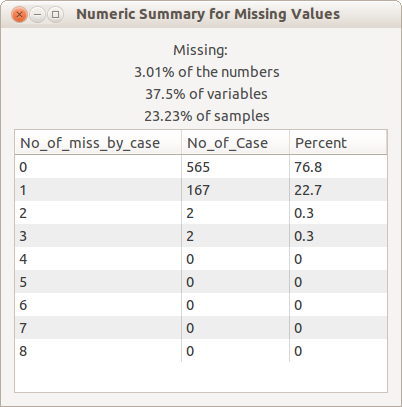
\includegraphics[width=0.33\textwidth]{graph/fig2-summary-1}
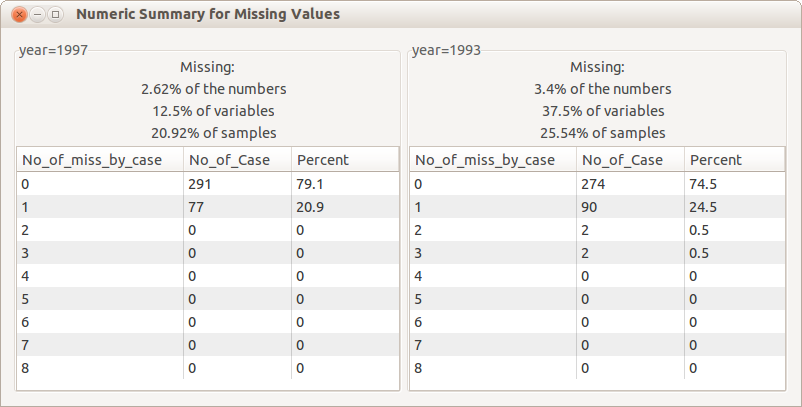
\includegraphics[width=0.66\textwidth]{graph/fig2-summary-2-condition}
\par\end{centering}
\caption{A numerical summary of missing values in the data is shown in a pop-up window. The left panel is given by unchecking any of the variables in region 2 of Figure~\ref{fig:missingGUI}. The percentages of missings by total number of data values, by variables and by cases, is shown on the top. This dataset has 8 variables and the missing values across variables is summarized in the bottom table. No cases have more than 3 missing values.  76.8\% of cases are complete, 22.7\% of cases have one missing value, and only 4 cases have more than one missing values. The right panel has the conditioning variable ``year'' checked in region 2, and provides the similar summaries for every category of the variable year.}
\label{fig: num-summry}
\end{figure}
\par\end{center}

\subsection{Imputation}\label{imputation}

A number of imputation methods are available in the package. The purpose of these is not only to examine the dependence between missings or non-missings, but also to produce a complete data set for later analysis. A few criteria were considered to improve user experience: (1) easy to understand and implement; (2) computing complexity is medium or low; (3) adaptability to different situations, i.e., not need strong model assumptions.

The seven imputation methods provided are: 
``Below 10\%'', ``Simple'', ``Neighbor'', ``MI:areg'', ``MI:norm'', ``MI:mice'', ``MI:mi''. 
In fact, ``Simple'' and ``Neighbor'' contains more than one method. As shown in Figure~\ref{fig:missingGUI} area 7, the three tab labels means three imputing methods provided by ``Simple'': overall median, mean/mode, and random value. ``Neighbor'' contains two methods: mean of the nearest neighbors, and random nearest neighbor. The neighbor methods allow the user to change the number of neighbors.

Table~\ref{tab:compare-methods} compares all the methods.

\begin{center}
\begin{table}[h]
\begin{centering}
\begin{tabular}{l|l|c|c|c}
\hline 
\textbf{\scriptsize{Method}} & \textbf{\scriptsize{Description}} & \textbf{\scriptsize{Determinisitic}} & \textbf{\scriptsize{Univariate}} & \textbf{\scriptsize{Multiple imp.}}\tabularnewline
\hline 
{\scriptsize{Below 10\%}} & {\scriptsize{below 10\% of the range}} & {\scriptsize{yes}} & {\scriptsize{yes}} & \tabularnewline
\hline 
 & {\scriptsize{overall median}} & {\scriptsize{yes}} & {\scriptsize{yes}} & \tabularnewline
{\scriptsize{Simple}} & {\scriptsize{overall mean/mode}} & {\scriptsize{yes}} & {\scriptsize{yes}} & \tabularnewline 
 & {\scriptsize{random value}} &  & {\scriptsize{yes}} & \tabularnewline
\hline
{\scriptsize{Neighbor}} & {\scriptsize{mean of the nearest neighbors}} & {\scriptsize{yes}} &  & \tabularnewline
 & {\scriptsize{random nearest neighbor}} &  &  & \tabularnewline
\hline 
{\scriptsize{MI:areg}} & {\scriptsize{predictive mean matching}} &  &  & {\scriptsize{yes}}\tabularnewline
\hline 
{\scriptsize{MI:norm}} & {\scriptsize{multivariate normal model}} &  &  & {\scriptsize{yes}}\tabularnewline
\hline 
{\scriptsize{MI:mice}} & {\scriptsize{multivariate imp. by chained equations}} &  &  & {\scriptsize{yes}}\tabularnewline
\hline 
{\scriptsize{MI:mi}} & {\scriptsize{multiple iterative regression imputation}} &  &  & {\scriptsize{yes}}\tabularnewline
\hline 
\end{tabular}
\par\end{centering}
\caption{Comparison among the methods. ``Deterministic''
means whether the result is deterministic or random. ``Univariate''
means whether the imputation only uses the individual variable where
imputation is needed, or makes use of other variables as well. ``Multiple
imp.'' indicates whether the methods is a type of multiple imputation.}
\label{tab:compare-methods}
\end{table}
\par\end{center}


\subsubsection{Univariate imputations}

The simplest example is setting the missing values to 10\% below the minimum of each variable. The purpose of this approach is to demonstrate the missing values in a place where they can be distinguished from the non-missing values. In a scatterplot, all missing values will lie along a vertical line on the left or a horizontal line on the bottom of the display (Figure~\ref{fig:univariate-imputation} (a)). In the histogram, missing values will form a bar to the left of other data values. And in the parallel coordinates plot, the missing values are at the bottom of each axis.

Using the median, mean, or mode of the complete cases is a common way to impute missing values. The median of a categorical variable is defined as the the most frequent category. With the mean/mode method, the missing values of a continuous variable are imputed by the mean of the complete cases, and that of a categorical variables will be imputed by the mode, i.e., the most common category. In the graph, points and bars are colored according to the missing status of the case. Figure~\ref{fig:univariate-imputation} (b) and (c) give an example of the imputation by median and mean for real-valued variables.

The ``random value'' method (Figure~\ref{fig:univariate-imputation} (d)) randomly selects an existing value of the variable to impute the missing. If there are more than one missing values in an observation, then they will be imputed respectively.

Because the above imputation methods operate separately on each variable, the dependencies between variables are ignored, and probably the methods will give biased covariance and correlation estimates. This is an issue in some circumstances, but sometimes it can be treated as a convenient and efficient way to visualize the missing values versus non-missings, standing up with other accurate but complicated methods. Inversely, a good visualization could help to check whether the univariate substitution is reasonable.


\begin{center}
\begin{figure}[h]
\begin{centering}
\begin{tabular}{cccc}
{\tiny{(a) Below 10\%}} &  &  & {\tiny{(b) Overall median}}\tabularnewline
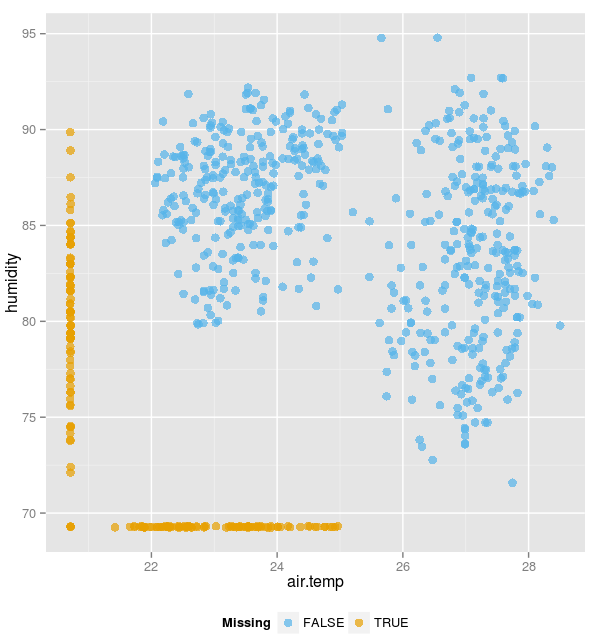
\includegraphics[width=0.32\textwidth]{graph/fig3-1-below10} &  &  & 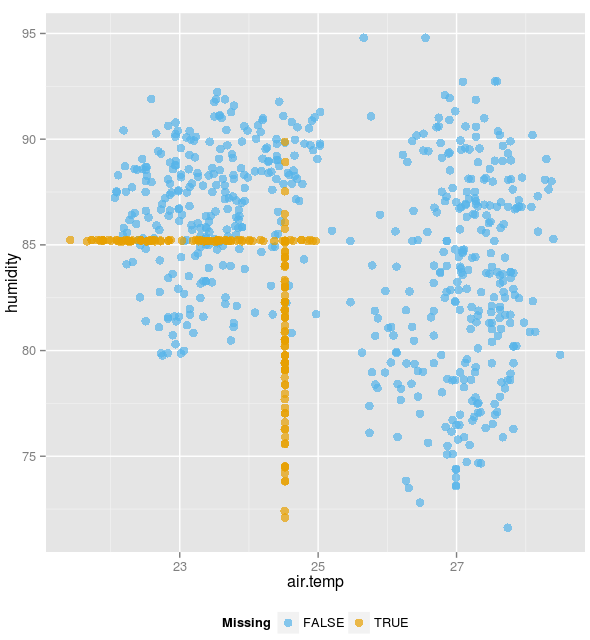
\includegraphics[width=0.32\textwidth]{graph/fig3-2-median}\tabularnewline
{\tiny{(c) Overall mean}} &  &  & {\tiny{(d) Random value}}\tabularnewline
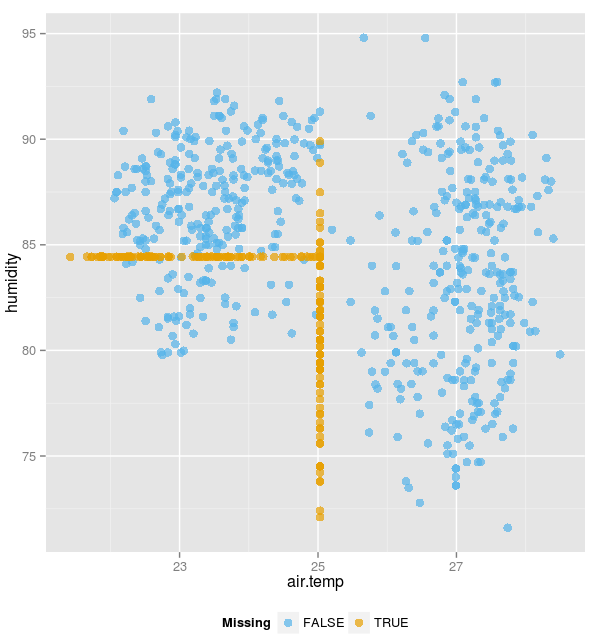
\includegraphics[width=0.32\textwidth]{graph/fig3-3-mean} &  &  & 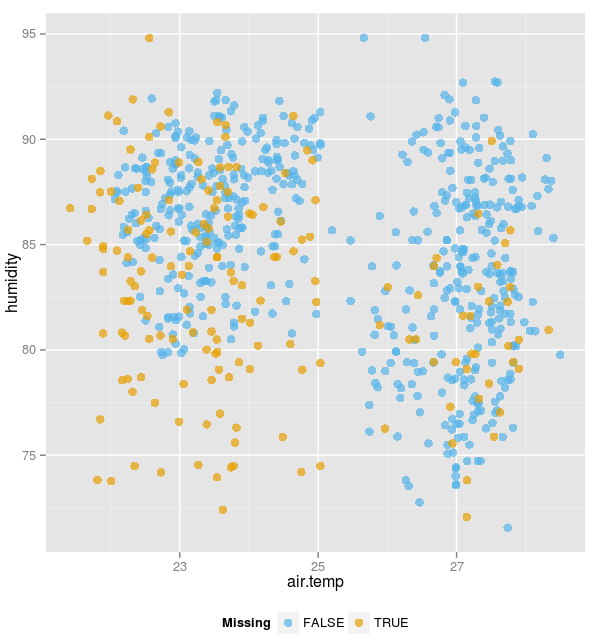
\includegraphics[width=0.32\textwidth]{graph/fig3-4-random}\tabularnewline
\end{tabular}
\par\end{centering}
\caption{Four panels of scatterplots displaying the results of different univariate imputations: (a) 10\% below the minimum (not strictly an imputation method, it is used more for displaying missings as part of a plot of complete cases); (b) median of each variable; (c) mean of each variable; (d) random selection from the existing values.}
\label{fig:univariate-imputation}
\end{figure}
\par\end{center}


\subsubsection{Neighbor imputations}

The ``Neighbor'' methods replaces a missing value with the mean or a random value of its $k$ nearest complete neighbors (Figure~\ref{fig:neighbor-imputation}). The distance between two observations is the Euclidean distance on the standardized variables that have no missings. Figure~\ref{fig:neighbor-diagram} explains the procedure. Ties are not considered, and only the first $k$ entries are used. This method requires at least one case in the dataset to be complete, and no character variables (ordinal variables are treated as integers). If there are less than $k$ complete cases, then all of them are used to generate the mean or a random value. If none of the cases are complete, then the mean or a random value of the entire data will be returned. $k$ is editable, and by default $k=5$.

The neighbor methods in \pkg{MissingDataGUI} can be seen as two special cases of hot deck imputation \citep{andridge2010review}. The neighbor mean method averages the weights on all chosen neighbors, and the random neighbor method places all the weights on one arbitrary neighbor. When $k=1$, the methods are deterministic hot deck.

%The methods should work well when the set of complete observations is large, but when there are few fully observations, the imputation may be biased due to too much waste information. 

\begin{center}
\begin{figure}[h]
\begin{centering}
\begin{tabular}{cccc}
{\tiny{(a) Mean of the neighbors}} &  &  & {\tiny{(b) Random neighbor}}\tabularnewline
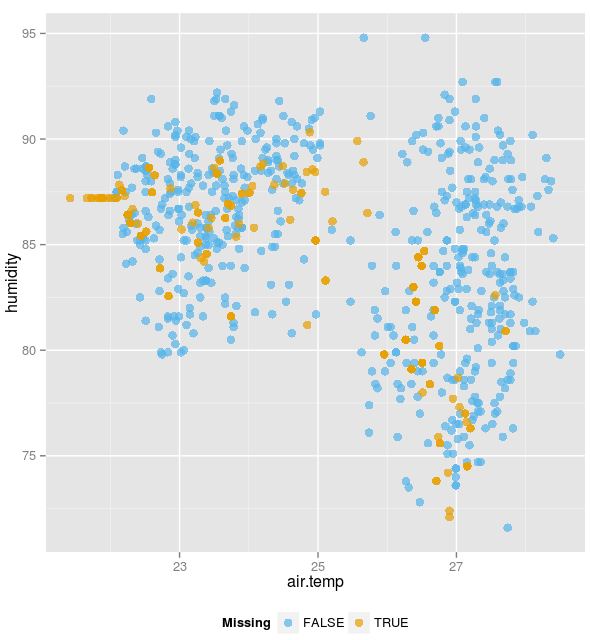
\includegraphics[width=0.32\textwidth]{graph/fig3-5-knn} &  &  & 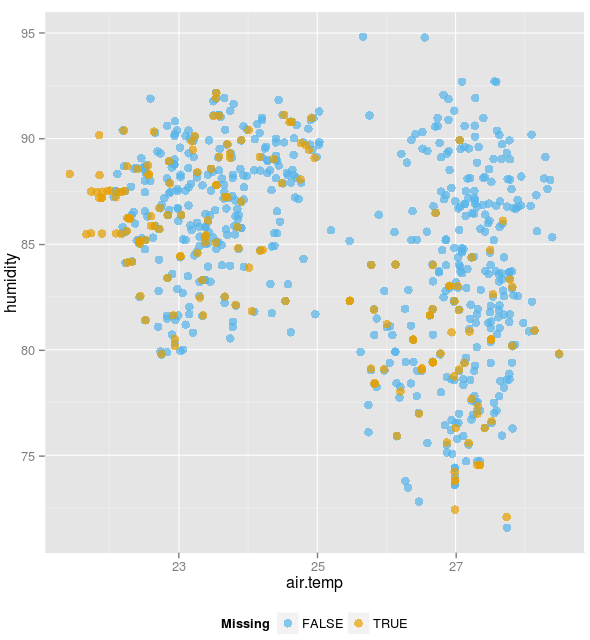
\includegraphics[width=0.32\textwidth]{graph/fig3-5-knn-2}\tabularnewline
\end{tabular}
\par\end{centering}
\caption{Scatterplots for two neighbor imputation methods. (a) mean of the 5 nearest neighbors; (b) a random value from the 5 nearest neighbors.}
\label{fig:neighbor-imputation}
\end{figure}
\par\end{center}


\begin{center}
\begin{figure}[h]
\begin{centering}
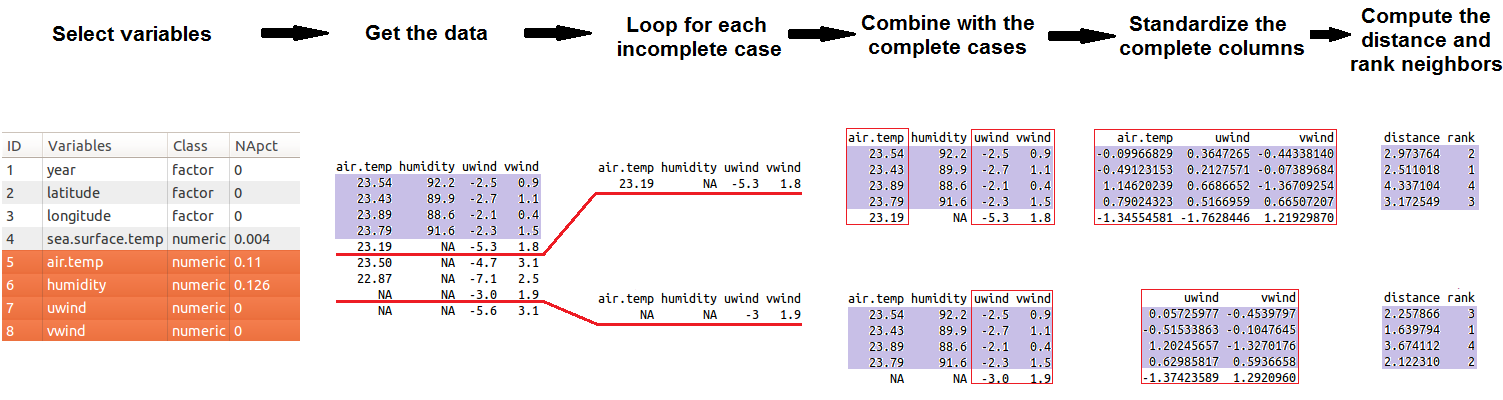
\includegraphics[width=1\textwidth]{graph/fig9-diagram}
\par\end{centering}
\caption{Illustration of the way to get $k$ nearest neighbors. The shaded entries are the complete observations to rank. The red frames circle the variables to compute the distance. After getting the rank of all complete observations, the first $k$ are used as neighbors. }
\label{fig:neighbor-diagram}
\end{figure}
\par\end{center}


\subsubsection{Multiple imputations}

Multiple imputation, first proposed by \citet{rubin1978multiple}, is a method to get valid inferences by the simulation approach. Multiple imputed datasets are generated based on the joint distribution to serve a wide variety of analytical goals.

As introduced in Section \ref{introduction}, four \proglang{R} packages are utilized to implement multiple imputations. Figure~\ref{fig:multiple-imputation} demonstrates the results of four packages on the same data. 

\begin{center}
\begin{figure}[h]
\begin{centering}
\begin{tabular}{cccc}
{\tiny{(a) \pkg{Hmisc}: predictive mean matching}} &  &  & {\tiny{(b) \pkg{norm}: multivariate normal model}}\tabularnewline
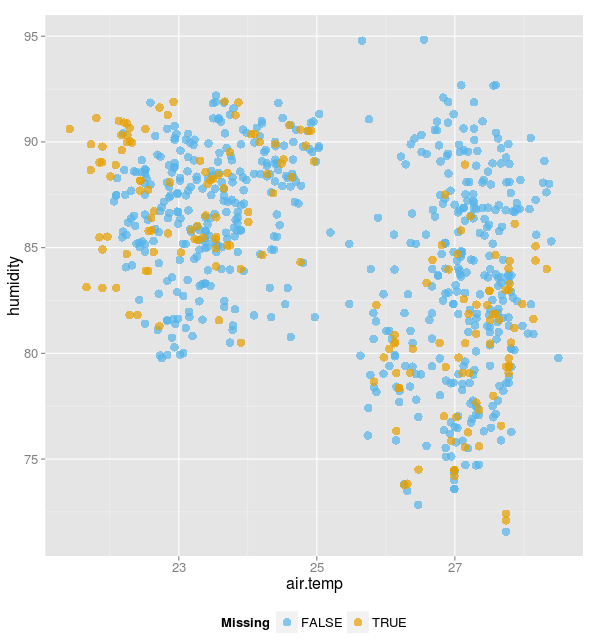
\includegraphics[width=0.32\textwidth]{graph/fig3-6-areg-2} &  &  & 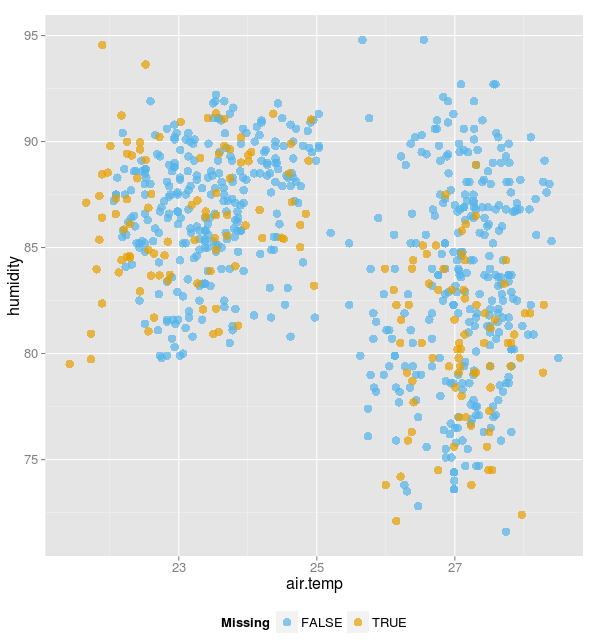
\includegraphics[width=0.32\textwidth]{graph/fig3-7-norm-2}\tabularnewline
{\tiny{(c) \pkg{mice}: chained equations}} &  &  & {\tiny{(d) \pkg{mi}: iterative regression}}\tabularnewline
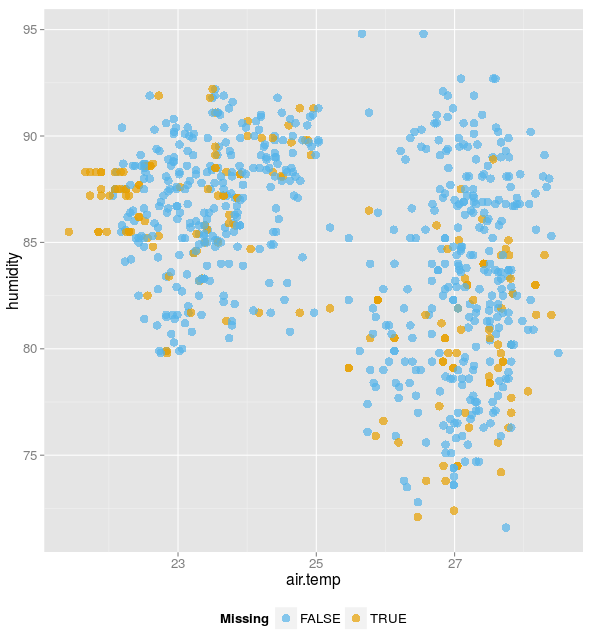
\includegraphics[width=0.32\textwidth]{graph/fig3-8-mice-2} &  &  & 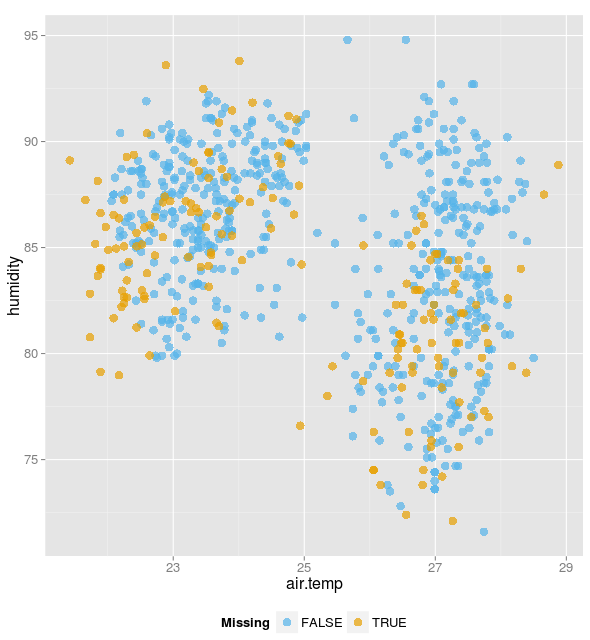
\includegraphics[width=0.32\textwidth]{graph/fig3-9-mi-2}\tabularnewline
\end{tabular}
\par\end{centering}
\caption{Scatterplots for the multiple imputations from four \proglang{R} packages: (a) predictive mean matching by \pkg{Hmisc}; (b) multivariate normal model by \pkg{norm}; (c) multivariate imputation by chained equations by \pkg{mice}; (d) multiple iterative regression imputation by \pkg{mi}. All the four plots are conditioned on year.}
\label{fig:multiple-imputation}
\end{figure}
\par\end{center}

Within the four packges, \pkg{norm} is very different from the other three. \citet{schafer1998multiple} introduced the basic idea of \pkg{norm}. It assumes the observations are sampled from a multivariate normal distribution, and uses EM algorithm to estimate the mean and variance-covariance matrix. Then it utilizes data augmentation method to converge the distribution. 

All the other three packages are using the chained equation approach with similar steps and slightly different settings. A comparison between the three packages is stated in Table~\ref{tab:compare-mi}, based on \citet{hmisc}, \citet{mice}, and \citet{mi}. The main differences are that \pkg{Hmisc} does not allow flexible models, and applies the bootstrap approach to obtain a sample for every iteration; \pkg{mi} utilizes a different criterion to check the convergency, as well as several new features for some special situations; \pkg{mice} stands in the middle of the other two: the models provided are more flexible than \pkg{Hmisc}, but not as bayesian as \pkg{mi}.

\begin{center}
\begin{table}[h]
\begin{centering}
\begin{tabular}{l|c|c|c}
\hline 
\textbf{\scriptsize{Algorithm}} & \textbf{\scriptsize{Hmisc}} & \textbf{\scriptsize{mice}} & \textbf{\scriptsize{mi}}\tabularnewline
\hline 
\textbf{\scriptsize{1. fill in the missing}} & \multicolumn{3}{c}{{\scriptsize{at random}}}\tabularnewline
\hline 
\textbf{\scriptsize{2. specify the model}} & {\scriptsize{pmm / regression}} & \multicolumn{2}{c}{{\scriptsize{user-specific model for each incomplete variable}}}\tabularnewline
\hline 
\textbf{\scriptsize{~~~~(default model)}} & \multicolumn{2}{c|}{{\scriptsize{predictive matching mean}}} & {\scriptsize{Baysian generalized linear models}}\tabularnewline
\hline 
\textbf{\scriptsize{3. decide the data}} & {\scriptsize{a bootstrap sample}} & \multicolumn{2}{c}{{\scriptsize{the entire dataset with the current imputed variable being non-missing}}}\tabularnewline
\hline 
\textbf{\scriptsize{4. iterate imputation}} & \multicolumn{3}{c}{{\scriptsize{in every cycle, variables with missings are imputed sequentially}}}\tabularnewline
\hline 
\textbf{\scriptsize{5. ``converge'' when}} & \multicolumn{2}{c|}{{\scriptsize{burning-in $k$ cycles}}} & {\scriptsize{difference of within and between variance is trivial}}\tabularnewline
\hline 
\end{tabular}
\par\end{centering}
\caption{Comparison among the multiple imputation packages using chained equation approach.}
\label{tab:compare-mi}
\end{table}
\par\end{center}

By default, $m=3$ chains are imputed and users can modify the number of chains. Each chain will produce a graphical panel in Figure~\ref{fig:missingGUI} area 7. Switching among the panels could compare the results by chain and any apparent discrepancy could be easily observed. Figure~\ref{fig:chaintabs} shows the results of four imputing chains by \pkg{mice}. 

\begin{center}
\begin{figure}[h]
\begin{centering}
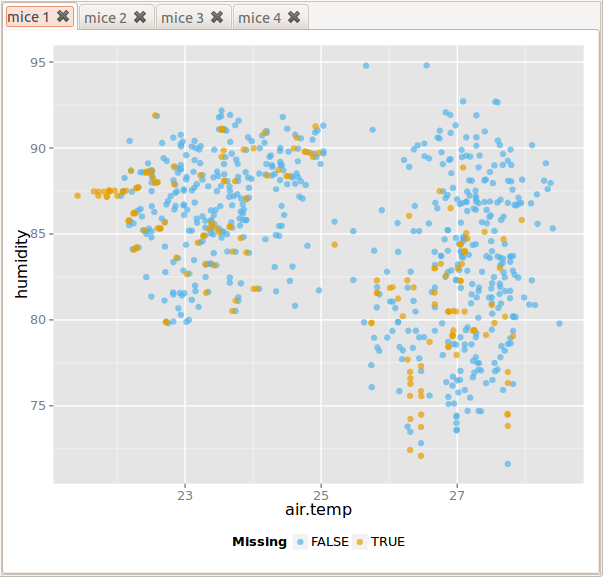
\includegraphics[width=0.24\textwidth]{graph/fig10-1-chain}
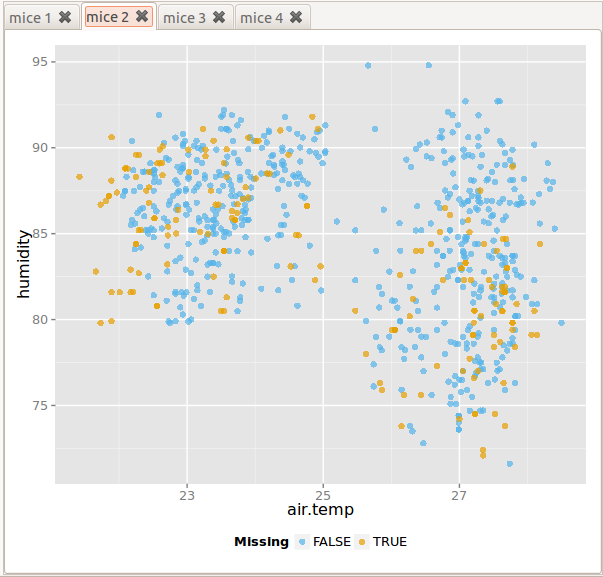
\includegraphics[width=0.24\textwidth]{graph/fig10-2-chain}
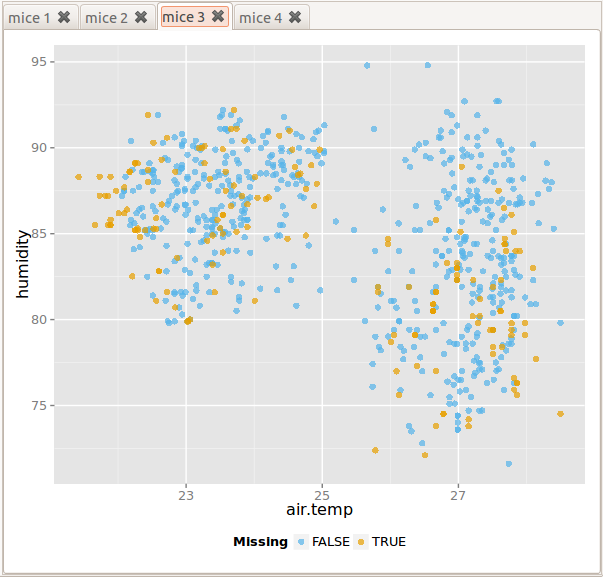
\includegraphics[width=0.24\textwidth]{graph/fig10-3-chain}
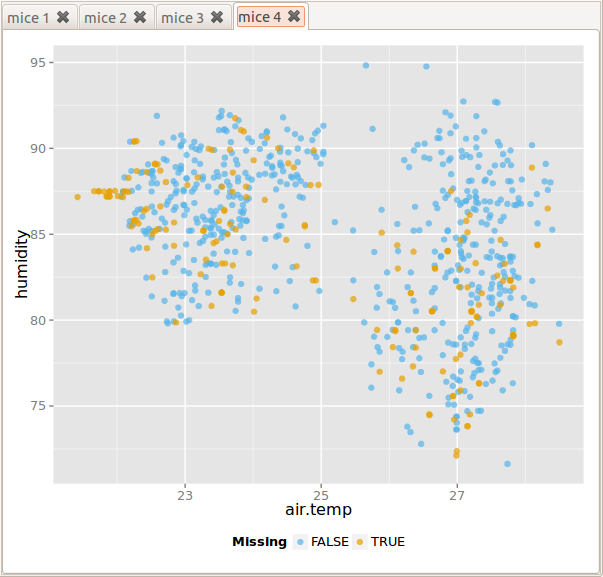
\includegraphics[width=0.24\textwidth]{graph/fig10-4-chain}
\par\end{centering}
\caption{Results of four imputing chains by \pkg{mice}, starting with the default random seed. Users can switch the panels by clicking the tabs, or close a panel by hitting the `x' sign. Focusing on the imputes at the left end, we see that the first, third and fourth chains cluster the imputes in a small range of y-axis, but the second chain spread them very evenly in the y-direction.}
\label{fig:chaintabs}
\end{figure}
\par\end{center}

\subsubsection{Conditional on the categorical variables}

When the variables of interest are bimodal or multi-modal, using the center statistics like mean or median as the imputations, or the simulation from an overall estimate like \pkg{norm}, is inadequate because the center can not reflect the shape of distribution properly. In many situations, the modalities arise from the mixture of groups. Hence, a better imputation method is to use the group means or medians instead of the overall mean or median.

The implementation of this idea produces the widget named ``categorical variables to condition on''. All categorical variables are listed with checkboxes. The variables checked will partition the data into blocks and then the imputation method is implemented in each block of the data. The procedure is as computing based on a conditional model given the category. However, the condition is invalid when the imputation method is ``Below 10\%'', since the aim of ``Below 10\%'' is only displaying the missings away from the non-missings, but giving the condition will mix the points again. If the conditioning factor variable has missing values, then a ``factor = NA'' group will be separated to calculate the numeric summary or the imputed values. If the conditioning factor itself is one of the plotting variables, then a message box will emerge to ask the user to impute the factor before other variables, and the plots are created without the condition.

The role of conditions in the imputation is revealed in Figure~\ref{fig: condition}. Without the condition, the imputations may locate far away from the distribution of values (Figure~\ref{fig: condition} left). But calculating separately by group provides a much better imputation (Figure~\ref{fig: condition} right).

\begin{center}
\begin{figure}[h]
\begin{centering}
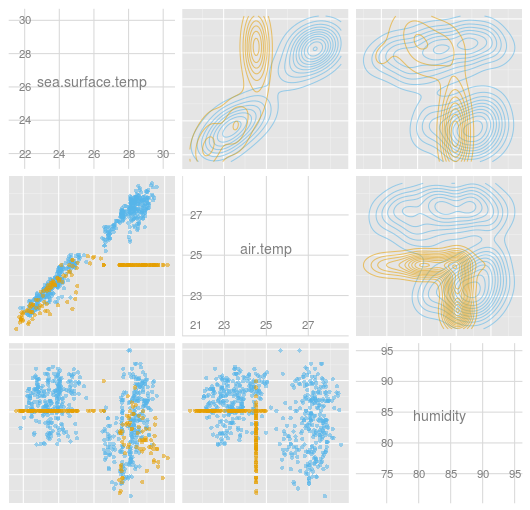
\includegraphics[width=.48\textwidth]{graph/fig4-1-median-uncondition}
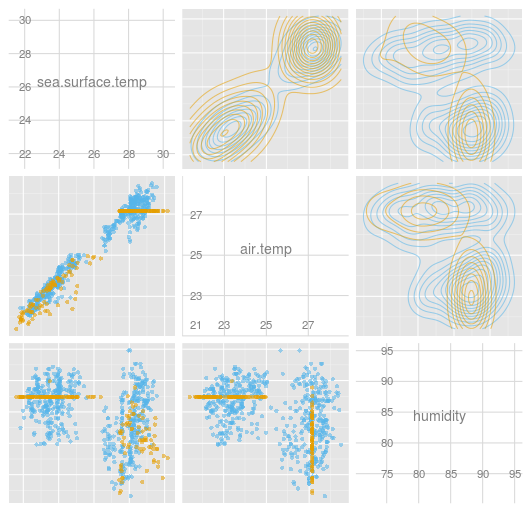
\includegraphics[width=.48\textwidth]{graph/fig4-2-median-condition}
\par\end{centering}
\caption{Comparison between imputations with and without conditions. The left panel is the imputation by median without condition and the right one is conditioned on year. In the left plot we can see that the imputed values fall between the two clusters, at the overall median. But when the imputation is conditioned on year (right plot), the imputed values are now better placed into the two clusters in the data.}
\label{fig: condition}
\end{figure}
\par\end{center}


\begin{center}
\begin{figure}[h]
\begin{centering}
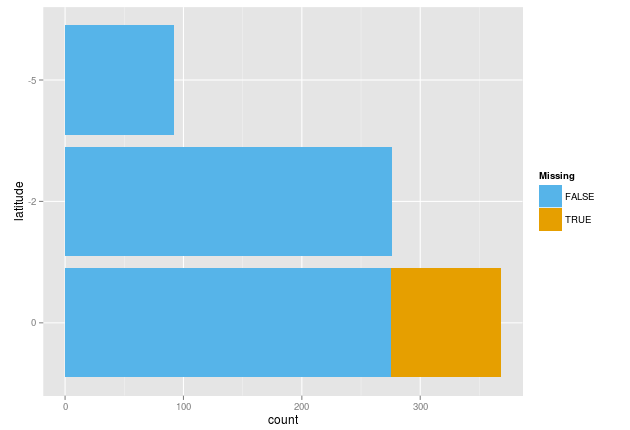
\includegraphics[width=.24\textwidth]{graph/fig5-1-barchart}
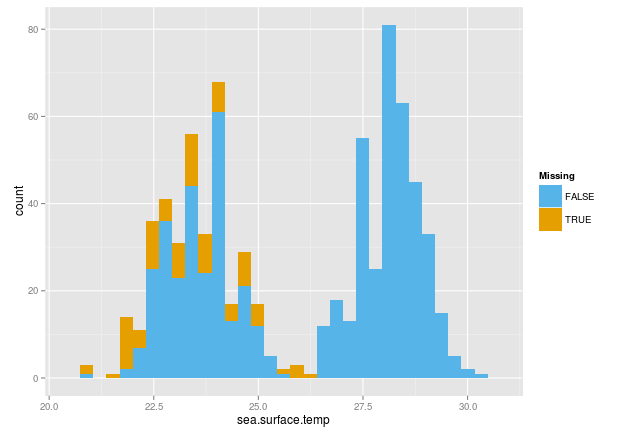
\includegraphics[width=.24\textwidth]{graph/fig5-1-histogram}
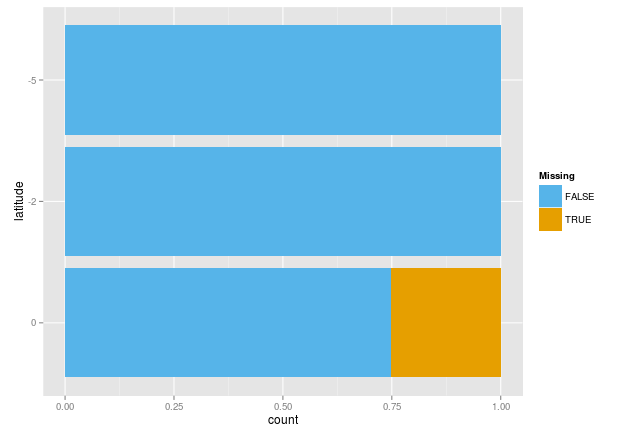
\includegraphics[width=.24\textwidth]{graph/fig5-1-spineplot}
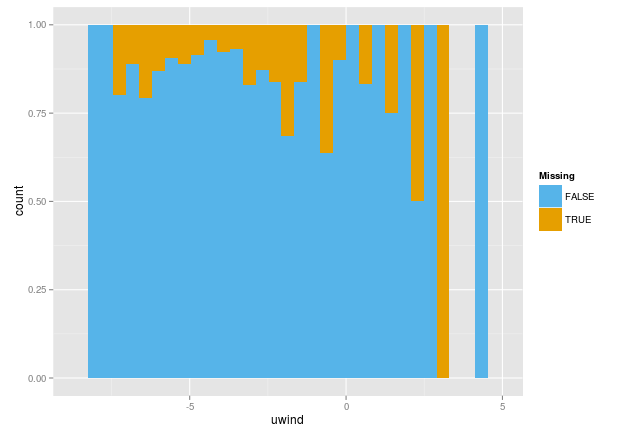
\includegraphics[width=.24\textwidth]{graph/fig5-1-spinogram}
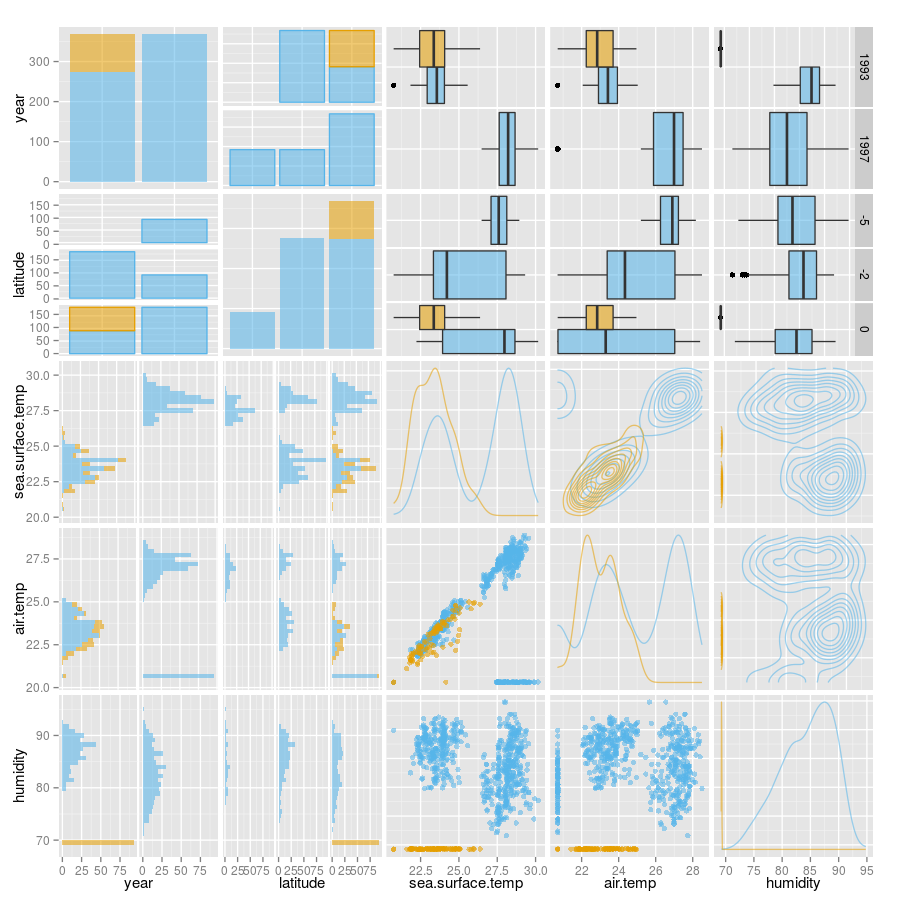
\includegraphics[width=.48\textwidth]{graph/fig5-2-pairwise}
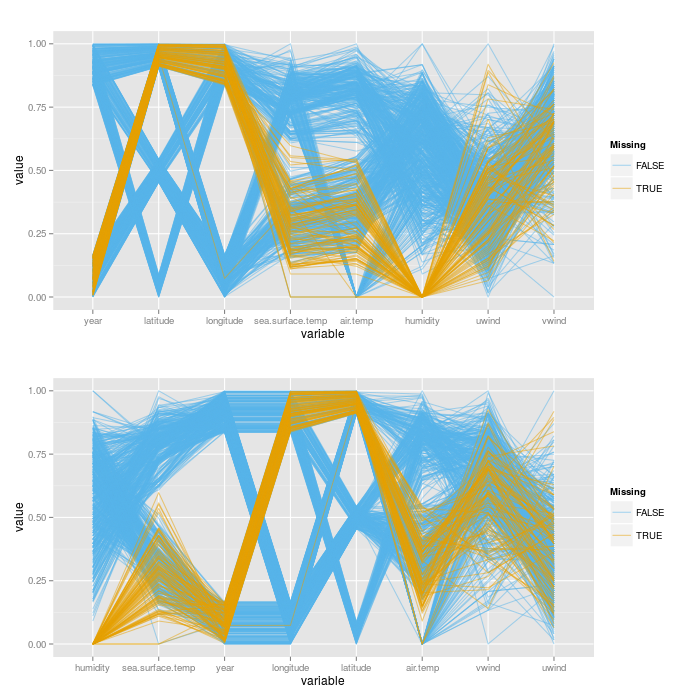
\includegraphics[width=.48\textwidth]{graph/fig5-2-pcp}
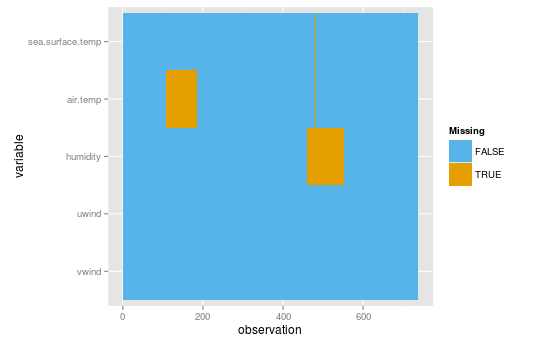
\includegraphics[width=.32\textwidth]{graph/fig5-3-map-1}
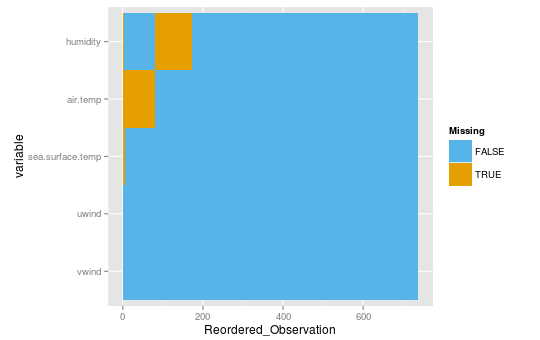
\includegraphics[width=.32\textwidth]{graph/fig5-3-map-2}
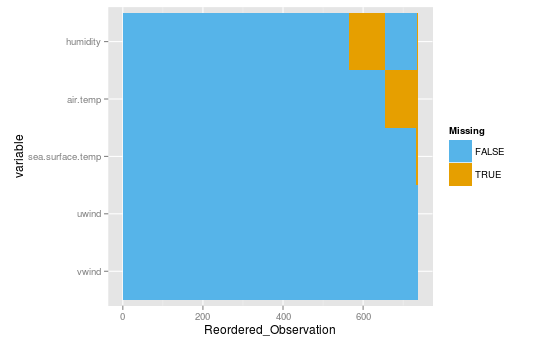
\includegraphics[width=.32\textwidth]{graph/fig5-3-map-3}
\par\end{centering}
\caption{Five types of graphs.
The first row from left to right are barchart, histogram, spineplot, and spinogram. The left panel on the second row are the pairwise plots, and the right shows two parallel coordinates plots. The order of variables is original on the upper plot, and on the lower one the variables separate the missing group and the complete group from the best to the worst. All the plots above use ``below 10\%'' imputation and color by the missing of one variable - humidity. The graphs on the third row are missingness maps with different orders of variables and cases. The left panel gives the original order; the middle one sorts the variables and cases by a decreasing number of missing values; the right one sorts them by hierarchical clustering of missingness.}
\label{fig:graphtypes}
\end{figure}
\par\end{center}

\clearpage

\subsection{Plot types}\label{plottype}

Five types of graphs are available in the missing data GUI: histogram (for continuous data)/ barchart (for categorical data), spinogram/spineplot, pairwise plots, parallel coordinates plot, and missingness maps. Figure~\ref{fig:graphtypes} displays all the graph types. Two color-blind friendly colors represent the observations and imputes on any variables that the user points to. In Figure~\ref{fig:graphtypes} the color means whether the value is originally missing in humidity, except for the missingness maps, where the yellow area indicates the missing values from any variable.

The histograms and barcharts are shown one by one for all the variables selected. When the missing values and the complete values share one bar, the bar is cut to two parts, and the ratio of two heights is equal to the ratio of missing and non-missing values in that bar. Besides, the histogram is laid vertically while barchart is horizontal, which will clearly differ the continuous and discrete data.

The spinograms (for continuous variable) and spineplots (for categorical variable), introduced by \citet{hummel1996linked} and \citet{theus1999visualizing}, are the scaled versions of histograms and barcharts, which provide a better visualization of the change of missing proportion upon the change of the observed values. In a spinogram/spineplot, each bar has the identical height, but is partitioned by two colors which represent the missing and non-missing values. The ratio of two heights is equal to the ratio of missings and non-missings too. Both histogram/barchart and spinogram/spineplot are generated via \pkg{ggplot2} \citep{ggplot2}.

Pairwise plots put the variable names and scales on the diagonal. For the continuous variables, the pairwise scatterplots are in the lower triangle. The upper triangle has two scenarios: one is the contour plots when all the selected incomplete variables are employed to color on; the other scenario is the correlation coefficients for the observations and imputes, when the imputed values are constant (e.g., by method ``Below 10\%'', overall mean, or overall median), and at least one selected incomplete variable is missed to color by (in this case the contour function does not work). For the categorical variables, barcharts by the categories of the vertical variable are given on both triangles. Again, the bars are colored in proportion to the missings. The combination of continuous and categorical variables is displayed as side-by-side boxplots of missing and non-missing values for each category on the upper triangle and side-by-side histograms on the lower triangle. Limited by the room of the graphics device in the main window, the pairwise plots cannot contain too many variables. The upper limit of the number of variables is set to be 5 and the lower limit is apparently 2. Function \code{ggpairs} from package \pkg{GGally} \citep{ggally} is in the use to draw the plots.

Parallel coordinates plot is originated by \citet{inselberg1985plane} to visualize high-dimensional data. In missing data GUI, all the selected variables are paralleled in two orders. One is the original order in the data frame; the other sorts the coordinates from the best separator to the worst by F statistic from ANOVA. A perfect separator could distinguish the imputes of the colored-by variable(s) completely from the observation. Hence under the ``Below 10\%'' setting, the selected incomplete variables should have higher power on separation; and by ``overall mean'' or ``Random Value'', the selected incomplete variables would have lower power. On the other hand, the selected variables without missing values should be marked if they have a higher rank on their separation capacity, because the observations are likely to be incomplete in a special area of these variables. Potentially the parallel coordinates plot may help to check the MCAR and MAR assumptions. By imputing the missing data with the ``Random Value'', we assume missing completely at random (MCAR). Additionally, if any conditioning factor variables were selected, then we assumed missing at random (MAR) conditioning on the factor. Cautions will raise if anything unusual happens in the link between the imputed variable and the covariates, for example, the yellow lines lie differently from the blue lines. The plots are produced by function \code{ggparcoord} from \pkg{GGally}.

The missingness map works as a graphical version of the shadow matrix, which provides an overview of the area of missing values in all variables. Assume that changing the order of variables and observations does not reduce any information, then agglomerating the missing values into blocks could enhance the understanding of missing patterns, especially for large data. Hence two re-ordered missingness maps are given besides the original map. One arranges the variables and cases by the number of missings, from the largest to the smallest; the other applies hierarchical clustering to both rows and columns.


\subsection{Design issues}
%\subsection{Maps to items in GUIs}

\begin{center}
\begin{figure}[h]
\begin{centering}
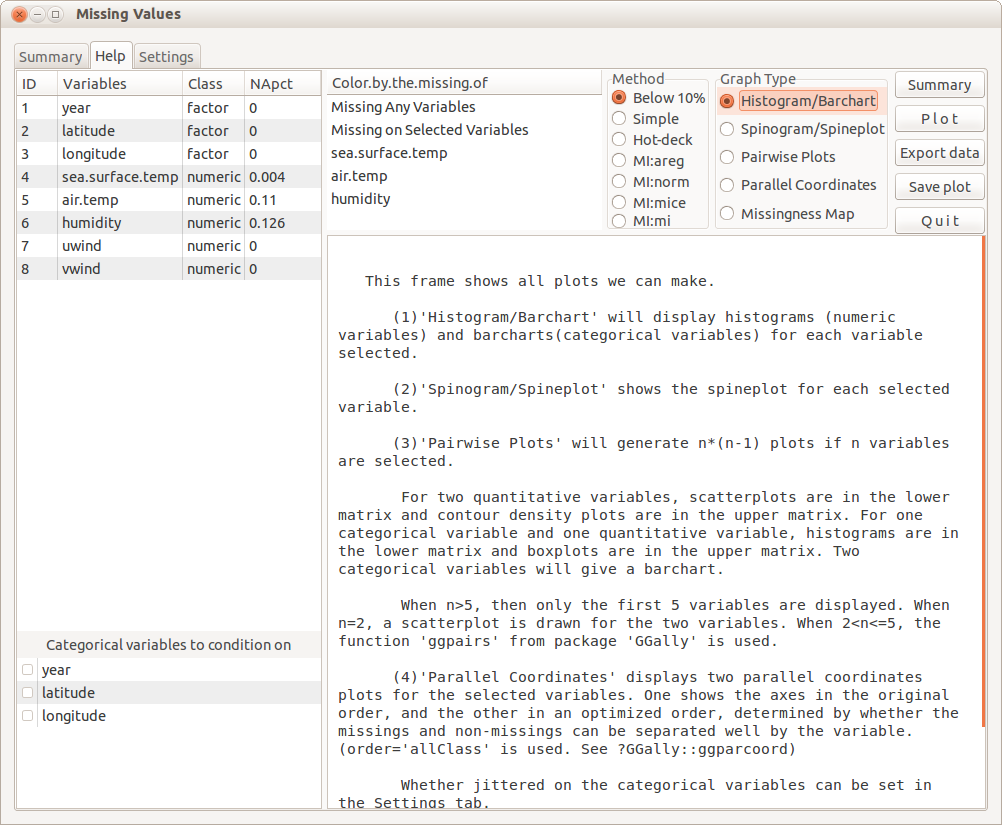
\includegraphics[width=0.9\textwidth]{graph/fig1-GUI-tab2}
\par\end{centering}
\caption{The help tab of missing data GUI. Mousing over any part of the GUI or clicking the radio/checkbox items will pop up text explanations in the summary region. All the widgets have their detailed introduction.}
\label{fig: missingGUI-help}
\end{figure}
\par\end{center}

The missing data GUI is designed in one window and three tabs. As shown in Figure~\ref{fig:missingGUI}, the summary tab includes all the important widgets: list of variables, radio for imputation methods, checkboxes for the conditional variables, the graphics device, etc.. An appropriate layout makes the widgets look not crowded, but very easy to maintain. The other two tabs are not as critical as the main tab, but also play important roles.

The help tab shown in Figure~\ref{fig: missingGUI-help} has the same layout as the summary tab. The only difference is that the graphics device is replaced by the help document. The corresponding help shows up when the user moves the mouse upon a widget. Compared to typing the question mark on the console and reading a literal instruction of the widgets, users could learn the GUI more quickly by this design.

The setting tab shown in Figure~\ref{fig: missingGUI-setting} provides the options 
of the imputation models in package \pkg{mice}, as well as other settings for 
the multiple imputation, neighbor selection, and display of parallel 
coordinates plot. To change the imputation models, users can double click a 
variable in the left table, and select any method provided in the pop-up window. 
The model candidates vary due to the class of the variable.

\begin{center}
\begin{figure}[h]
\begin{centering}
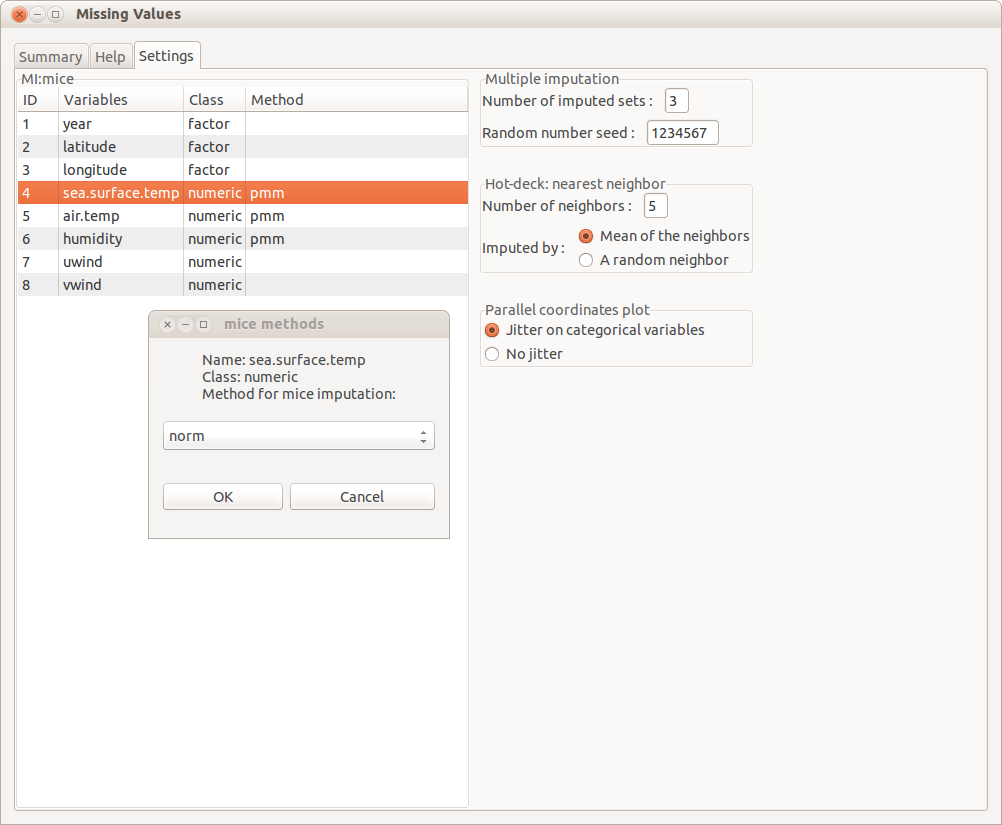
\includegraphics[width=0.9\textwidth]{graph/fig1-GUI-tab3}
\par\end{centering}
\caption{The setting tab of missing data GUI. Variables are listed with their classes in the left table. The fourth column gives the current \pkg{mice} methods for all incomplete variables. On the right users can modify the number of imputed sets, random number seed, the number of neighbors, and the jitter setting for parallel coordinates plot.}
\label{fig: missingGUI-setting}
\end{figure}
\par\end{center}


\subsection{Data input and output}

Data can be read in as either a data frame or a comma separated values (csv) file. The preferred approach is to read an existing data frame in \proglang{R} because the type of variables (factor, numeric, ...) are reserved. \code{MissingDataGUI(data)} is the starting function in this case.

Reading from a csv file is another choice.  If \code{MissingDataGUI()} is called without a data frame argument, data import GUI is called (Figure~\ref{fig: import}). The ``Open'' button is for choosing files and the ``Watch Missing Values'' buttons will launch the missing data GUI. The file format must be csv currently, and only one data set can be imported every time, though more than one file can be opened in the data import GUI.

\begin{center}
\begin{figure}[h]
\begin{centering}
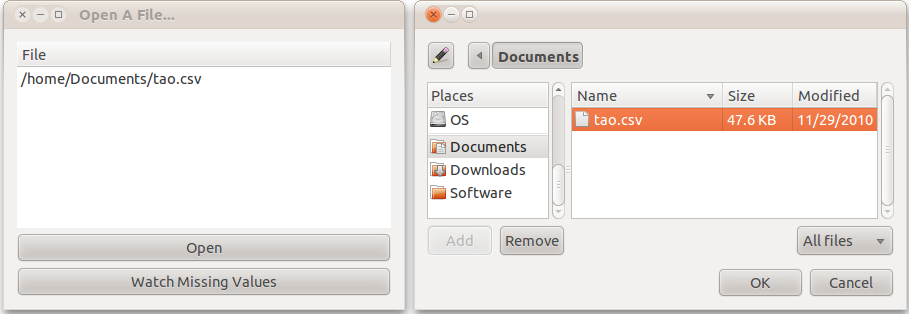
\includegraphics[width=0.9\textwidth]{graph/fig6-open}
\par\end{centering}
\caption{The data import GUI, with file selector, which is called by the ``open'' button. More than one file could be listed in the GUI, but only one data set is allowed active. The first file is automatically imported if none of the data sets are chosen when the ``Watching Missing Values'' button is hit.}
\label{fig: import}
\end{figure}
\par\end{center}

The imputed data can be saved by the ``Export data'' button. Only the selected variables will be imputed, but users could choose whether to export the selected columns or all the columns (with \code{NA}'s existing in the unselected variables). The shadow matrix is exported by default, so that analysts can always track back to find the locations of the real missings. As seen in Figure~\ref{fig: export}, data could be saved in three ways: csv file, rda file, or a data frame in \proglang{R} console.

The exported data with its shadow matrix can be loaded back again to the GUI, which implies the imputed data from other imputation methods (not provided by the missing data GUI) can also be imported. Users only need to provide a shadow matrix which indicates the locations of missings. In other words, the imported structure should be a data frame or a csv file with the first $n$ columns being the imputed data and the next $n$ columns being the shadow matrix. In this situation, ``Below 10\%'' method will generate the graphs from the imported data, instead of the actual ``Below 10\%'' imputation.

\begin{center}
\begin{figure}[h]
\begin{centering}
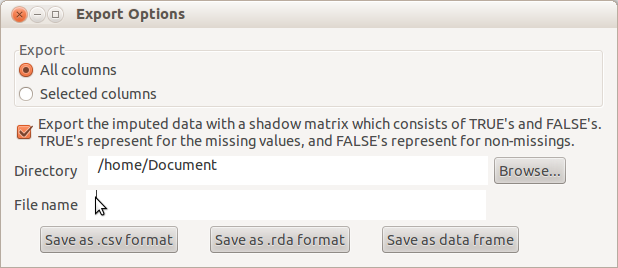
\includegraphics[width=0.6\textwidth]{graph/fig7-export}
\par\end{centering}
\caption{The data export GUI. By default, all columns are exported with a shadow matrix. The current working directory is set to be the default. Three exporting formats are provided.}
\label{fig: export}
\end{figure}
\par\end{center}


\subsection{Additional features of the GUI}

\begin{itemize}
\item Change the attributes. Double clicking on any variables in the top left table of the summary tab will open an attribute window, as displayed in Figure~\ref{fig: attributes}. Users could edit the variable name, or assign another class to the variable. When the class of a variable is switched from numeric/integer to character/factor/ordinal, the variable will be automatically loaded into the checkbox group as the potential conditions.

\begin{center}
\begin{figure}[h]
\begin{centering}
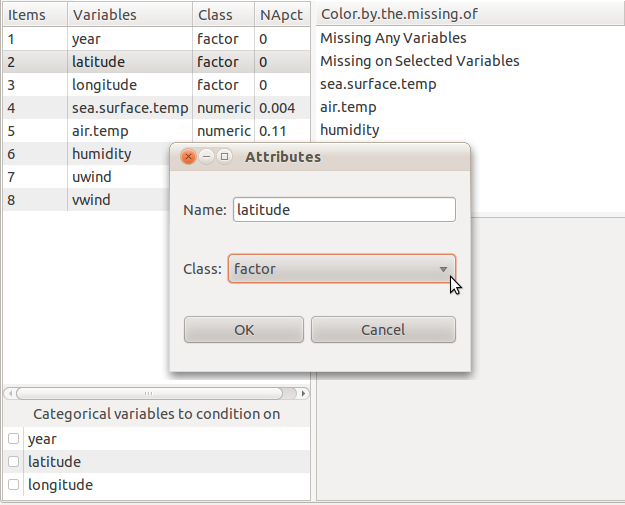
\includegraphics[width=0.6\textwidth]{graph/fig8-query}
\par\end{centering}
\caption{The attributes list for variable selection is interactive. The name can be edited, and the class could be changed to one of the five classes: integer, numeric, character, factor, or ordinal (factor). When a numeric variable is changed to a categorical variable, the widget for conditions will be updated.}
\label{fig: attributes}
\end{figure}
\par\end{center}

\item Search a variable by typing. The variable table, conditioning checkboxes, and color-by-variable selector allow text entry to find a variable. This feature is especially useful when there are plenty of variables in the data.
\item Save the plots. Plots can be saved tp png files by ``Save plot'' button. The imputation method and plot type will be auto-completed in the file name. All of the figures in the Example section were saved this way.
\end{itemize}


\section{Examples}\label{Examples}

\subsection{Data}

Two data sets are provided with the package: \code{tao}, which is used as the example in this paper, and \code{brfss}. \code{brfss} is a subset of the 2009 survey from the Behavioral Risk Factor Surveillance System, an ongoing data collection program designed to measure behavioral risk factors for the adult population (18 years of age or older) living in households. The website for this program is \url{http://www.cdc.gov/BRFSS/index.htm}.

\code{tao} is from the Tropical Atmosphere Ocean project (TAO) \citep{tao}. The TAO array consists of approximately 70 moorings in the Tropical Pacific Ocean, telemetering oceanographic and meteorological data to shore in real-time via the Argos satellite system. A subset of data from 6 moorings in 1993 and 1997 is used for the example. The data has 8 variables (year, latitude, longitude, sea surface temperature, air temperature, humidity, uwind and vwind) and 736 observations. This subset is provided by \citet{CS07}. We can open the GUI by the following commands:

\begin{Code}
library("MissingDataGUI")
MissingDataGUI(tao)
\end{Code}

The numeric summary of all 8 variables in this data is shown in Figure~\ref{fig: num-summry}.

%The access to data is as Figure~\ref{fig: import} and by clicking the button ``Watch Missing Values'' in the data import GUI we will get Figure~\ref{fig: missingGUI} without activating the graphics device. 


\subsection{Exploring missings}

Three of the 8 variables have missing values. First let's look at the distribution of missings on these variables. Figure~\ref{fig:tao1} (left) shows the pairwise plots of these three variables with any missing values colored in yellow. Cases which are missing on humidity have low values of sea and air temperature. This suggests the dependence between humidity missingness and the temperature variables. Imputation methods that incorporate this dependence may be preferable.

Figure~\ref{fig:tao1} (right) shows the data imputed with median values (yellow). This imputation imposes a cross structure on the data, which does not match the shape of the complete cases. For example, there is a line of imputed values in the plot of air temperature versus sea surface temperature which is far from the rest of the complete cases. Thus the imputation method does not work well for this data.

Figure~\ref{fig:tao3} (left) shows the data conditional imputing with median values (yellow) by year. This better matches the distribution of complete cases, although the imputed values still form bands in the scatterplot. This might be a problem because the variance estimation will be affected. 


\begin{figure*}[htp]
\centerline{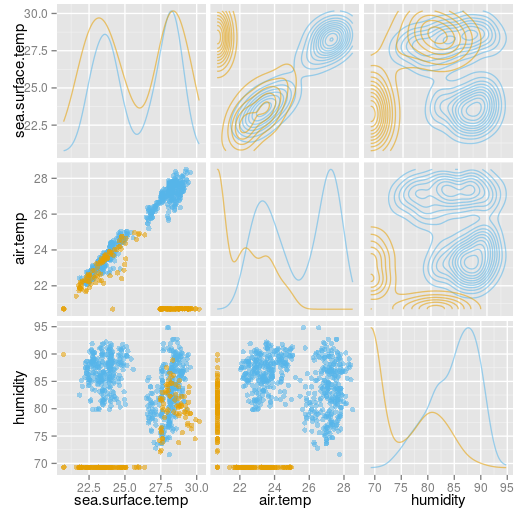
\includegraphics[width=0.49\textwidth]{graph/fig4-3-below10-uncondition}
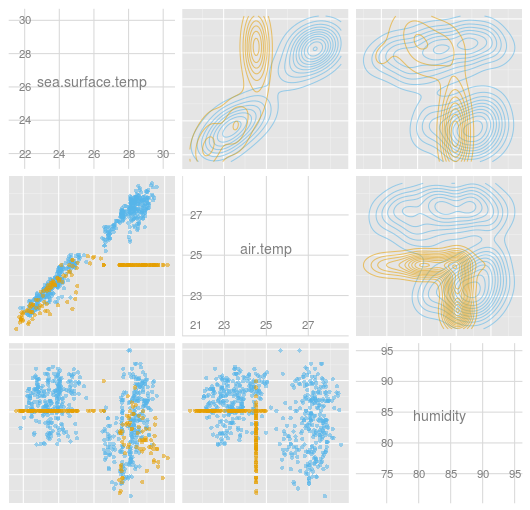
\includegraphics[width=0.49\textwidth]{graph/fig4-1-median-uncondition}}
\caption{(Left) Exploring the effect missingness of humidity on sea and air temperature. Missings on humidity occur at the lower temperature values, suggesting a dependent relationship. Missing values are not missing completely at random. (Right) Exploring imputation methods. Imputation using the medians is shown here. Values that have been imputed are shown as yellow. Median imputation introduces a cross structure to the point scatter, and the imputed values don't match the data well, for example the line of imputed values is very apart from the complete cases in the plot of the tao temperature variables.}
\label{fig:tao1}
\end{figure*}

\begin{figure*}[htp]
\centerline{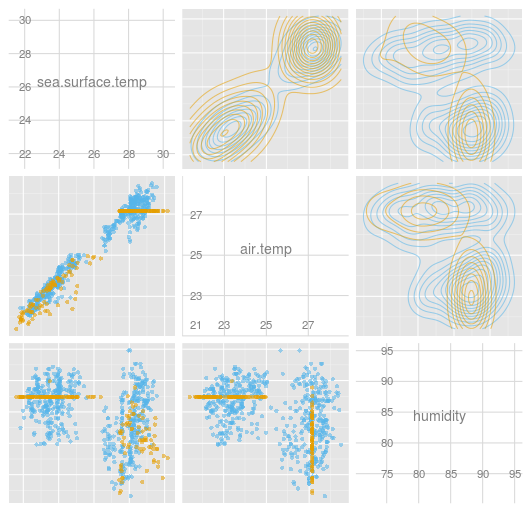
\includegraphics[width=0.49\textwidth]{graph/fig4-2-median-condition}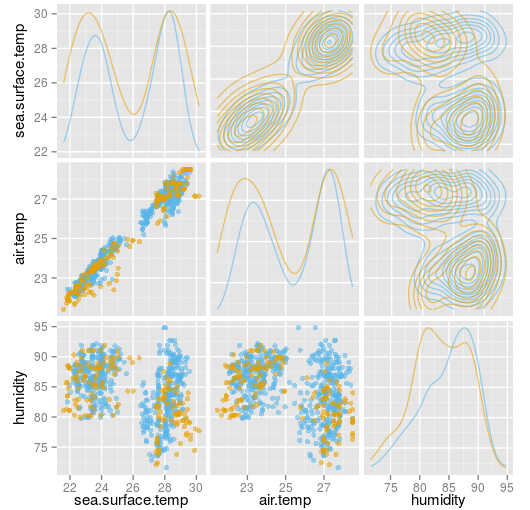
\includegraphics[width=0.49\textwidth]{graph/fig4-4-areg-condition}}
\caption{(Left) Imputation using the median conditional on year. Imputed values better match the complete cases, with the exception of the banding due to fixed median value. (Right) Imputation using the regression conditional on year. The distribution of imputed values is fairly close to the distribution of complete cases.}
\label{fig:tao3}
\end{figure*}

For this data, the better ways to impute the data would take the strong association between the variables into account. This suggests that neighbor or multiple imputation might be the more desirable imputation methods. Figure~\ref{fig:tao3} (right) shows the results for MI:areg, the regression-based imputation, conditional on year. The imputed values match the distribution of complete cases reasonably well. There are a few slight concerns: some of the imputed values have lower air temperature values than any of the complete cases, the spread of the imputed values is a little greater than the complete cases. But overall, this is probably as good as it is going to get with imputing the missings for this data set. It would be reasonable to export the imputed data for further analysis at this point.


\section{Discussion}

The main goal of this work is to make it possible to see the the missing data and the impact of various imputation methods. In the future interactive data visualization will make it possible to brush points in a plot to more completely explore missing structure as we can in \proglang{GGobi} and \proglang{MANET}.


\section*{Software}

This missing data GUI is written in \proglang{R} 3.0.2 \citep{r} and based on the package \pkg{gWidgets} \citep{gwidgets} with the toolkit \proglang{RGtk2}. 

On different platforms (Windows, Linux, Mac) the appearance of the GUI will differ slightly, but the functionality will be the same.

\section*{Acknowledgements}

This work was partially supported by an unrestricted fellowship from Novartis, and National Science Research grant DMS0706949.

\bibliography{MissingDataGUI}
\end{document}
